\documentclass[dvipdfmx]{jsarticle}
\usepackage[T1]{fontenc}
\usepackage[dvipdfmx]{hyperref}
\usepackage{lmodern}
\usepackage{latexsym}
\usepackage{amsfonts}
\usepackage{amssymb}
\usepackage{mathtools}
\usepackage{amsthm}
\usepackage{multirow}
\usepackage{graphicx}
\usepackage{wrapfig}
\usepackage{here}
\usepackage{float}
\usepackage{ascmac}
\usepackage{url}
\newtheorem{dfn}{定義}
\newtheorem{thm}{定理}

\title{解集合プログラミングを使用した宣言的問題解決に関する計算機実験}
\author{文理学部情報科学科\\5419045 高林 秀}
\date{\today}

\begin{document}

\maketitle

\begin{abstract}
本稿は、今年度論理と計算2における課題学習として「解集合プログラミング」及び「具体的な問題の解決を行う計算機実験」を行うものである。本稿の冒頭〜中盤では関係理論の説明を行い、終盤ではその理論を利用して、実際に具体的な問題に対する解答を提示する。なお、本演習にはソルバーとしてclingoを使用した。
\end{abstract}

\section{目的}
本稿は、今年度論理と計算2の課題研究として、解集合プログラミングを使用した宣言的問題の解決と、その関係理論の説明を通して講義内容を振り返るものである。\par
以降、本稿の概要は次のとおりである。
\begin{enumerate}
  \item 計算理論説明
  \begin{enumerate}
    \item 述語論理について
    \begin{enumerate}
      \item 構文
      \item 限量子
      \item 解釈とモデル
      \item 標準形
    \end{enumerate}
    \item 論理プログラムについて
    \begin{enumerate}
      \item エルブラン領域・基底
      \item 論理プログラムのクラス区分
      \item 確定論理プログラム
    \end{enumerate}
    \item 標準論理プログラムについて
    \item 安定モデルについて
    \begin{enumerate}
      \item 導出アルゴリズム
    \end{enumerate}
    \item 解集合プログラミングについて
  \end{enumerate}
  \item 計算機実験
  \begin{enumerate}
    \item clingoの説明
    \item ハミルトン経路
    \item 数独
  \end{enumerate}
  \item 各問に関する考察
  \item まとめ
  \item 巻末資料
\end{enumerate}
\section{計算理論説明}
この章では、今回の計算機実験に使用した各計算理論の解説を行う。
\subsection{述語論理について}
ここでは論理プログラムに入る前に前提知識となる、述語論理に関する説明を行う。前提となる命題論理に関する説明は下記URLから参照いただきたい。以下のレポートでは、原子文、複合文等基本用語についてまとめたものである。\par
\begin{itemize}
  \item 命題論理に関するレポート:\url{https://drive.google.com/drive/folders/1kOW_1KPUw_kBznaMWjge7HaBI7FoRAoq?usp=sharing}
\end{itemize}
述語論理とは、デジタル大辞泉によると以下のように書かれている。
\begin{quote}
  記号論理学の一部門。命題内部の論理構造である主語と述語の関係「すべての主語は…である」「ある主語は…である」などを、論理記号(全称∀・存在∃など)によって記号化して研究するもの
\end{quote}
これまで扱ってきた命題論理は、命題のみ扱うことができた。したがって、多数のオブジェクト\footnote{オブジェクト:主に名詞、またはそのかたまり(名詞句、名詞節)}間の関係性\footnote{オブジェクト間の関係:そのオブジェクトの動詞にあたるもの。}を記述することは難しく、それぞれの関係性ごとに逐一命題変数などを用意して記述する必要があった。より具体的には、命題論理はその命題の内容にかかかわらず真偽のみに着目する。各命題文同士の関係性を説明するとき、命題記号(命題変数)に変形し推論を行うので、その妥当性を評価するのがむずかしくなる。以下参考となるページのリンクを挙げる。
\begin{itemize}
  \item 論理学補足文書:\url{http://student.sguc.ac.jp/i/st/learning/logic/%E8%BF%B0%E8%AA%9E%E8%AB%96%E7%90%86.pdf}
\end{itemize}
上記ではこのことを「命題論理の限界」と説明しており、述語論理はそのような弱点を克服した上位の論理言語であると捉えることができる。\par
述語論理はその関係性に焦点をおいた論理言語で、オブジェクト間の関係性を簡単に示すことができる。また、命題論理では扱わなかった、推論の妥当性に関して扱うことができる。\par
述語論理は、以下のように区分けされている。
\begin{itemize}
  \item 一階述語論理:オブジェクトの変数化ができる。
  \item 二階述語論理:オブジェクトの変数化に加え、述語、関数記号の変数化ができる。
  \begin{itemize}
    \item 高階述語論理:引数として、1つ以上別の述語ないしは関数記号をとることができる。一般化すると、 $n$ 階述語の引数は1つ以上の ($n$ − 1) 階の述語である。
  \end{itemize}
\end{itemize}
以下、その表記の仕方と、登場する記号に意味について説明する。
  \subsubsection{構文}
  述語論理において、主語や目的語に相当するものを「対象」と呼ぶ。この「対象」は変数、定数のいずれでもよい。加えて、動詞や形容詞に相当するものを「述語」と呼ぶ。\par
  これらの語句を用いると、述語論理の表記は次のように表すことができる。
  \begin{itemize}
    \item 述語(対象,対象,...)
  \end{itemize}
  また、「対象」は「項(term)」とも言われ、項には定数、変数、関数記号が存在する。すなわち、述語、関数記号の引数に該当する。\par
  \paragraph{述語論理における関数}
  ここで「関数記号」というものが登場したがこれは、構造を持つような複雑なオブジェクトを形式的に示すものである。一般的な数学やプログラムの場合、関数記号は引数になにか入力が与えられ、何かしら結果を出力するものであるが、述語論理における「関数」はそれとは無関係である。つまり、単に1つの記号として扱われるということである。\par
  \paragraph{基礎項}
  変数を1つも含まない項を「基礎項」と呼ぶ。これは、具体的な項、すなわちオブジェクトを示す。
  \paragraph{基礎原子文(ground atom)}
  引数すべてが、基礎項であるような原子文(atom)、すなわち変数がない原子文を「基礎原子文」と呼ぶ。これは、真理値を割り当てる対象となる文である。\par

  1つ具体例を挙げる。次のような普通の文を考えてみる。
  \begin{itemize}
    \item 「地球と太陽は惑星である」
  \end{itemize}
  これを述語論理の形式で示すと以下のようになる。
  \begin{itemize}
    \item $orbits(earth, sun)$
  \end{itemize}
  この場合は、$orbits$(惑星である)という述語の目的語、すなわち対象として「$earth$(地球)」と「$sun$(太陽)」が割り当てられている。述語論理ではこの様な形式(述語文)を最小単位として、命題論理と同様の結合子を用いて、複合文を形成することもできる。
  \begin{table}[H]
    \centering
    \begin{tabular}{lll}
    記号                & 訳 & 意味\\
    $\wedge$          & 連言 & プログラミングではよくand、\&\&として扱われる。pかつq\\
    $\vee$            & 選言 & プログラミングではor, ||。pまたはq\\
    $\neg$            & 否定 & プログラミングではnot, !。pではない\\
    $\Rightarrow, \supset$     & 含意 &〜ならばの意味で使われる。\\
    $\Leftrightarrow, \equiv$ & 同値 &「pはqである」がtrueのとき、\\&&もしくはその時点に限りtrueであるとき。pとqは同値。\\
    $\top$ &トートロジー(恒真)&トートロジーを示す記号 \\
    $\bot$ &恒偽(矛盾)&恒偽を示す記号\\
    (補足)$\veebar, \oplus$ & 排他的論理和& NANDと呼ばれるもの。\\
    \end{tabular}
    \caption{主要な結合子}
\end{table}
命題論理のときと同様に、例えば「$have\_a\_fever(X)$(Xは熱を持っている)ならば$take\_a\_drag(X)$(Xは薬を飲む)」は、「$have\_a\_fever(X)\Rightarrow take\_a\_drag(X)$」というようにして2つの述語文をつなげることもできる。

  \subsubsection{限量子}
ここでは、命題論理には存在しない「限量子」という記号について扱う。限量子とは一言で言えば「変数の範囲を規定するもの」である。例えば、先程の例で$have\_a\_fever(X)$「Xは熱を持っている」としたが、この対象Xの範囲を規定する役割を果たす。\par
限量子には以下2種の記号が存在する。
\begin{itemize}
  \item 全称限量子:$\forall$:「すべての〜、任意の〜」というように全てが対象である事を示す。
  \item 存在限量子:$\exists$:「少なくとも1つの〜、ある〜に対して」というように、1つ以上の対象が存在することを示す。
\end{itemize}
より厳密に言うと、Wikipediaには以下のように書かれている。
\begin{itemize}
  \item 全称限量子:引用元\url{https://ja.wikipedia.org/wiki/%E5%85%A8%E7%A7%B0%E8%A8%98%E5%8F%B7}
  \begin{quote}
    全称記号(ぜんしょうきごう、universal quantifier)とは、数理論理学において「全ての」(全称量化)を表す記号である。通常「∀」と表記され、全称量化子(ぜんしょうりょうかし)、全称限量子(ぜんしょうげんりょうし)、全称限定子(ぜんしょうげんていし)、普遍量化子(ふへんりょうかし)、普通限定子(ふつうげんていし)などとも呼ばれる。
    \[中略\]
    「$Px$」という開論理式 (ope.sn formula) が与えられたとき、これが意味するところは「……はPである」ということだけで、これだけでは真偽が確定しない。\[中略\]
    このうち全称記号「∀」によって束縛した場合には「$\forall x Px$」という閉論理式が得られ、これは「全ての(任意の) $x$ について、$x$ は $P$ である」(より簡単には「全ての $x$ は $P$である」)という意味になる。
  \end{quote}
  \item 存在限量子:引用元\url{https://ja.wikipedia.org/wiki/%E5%AD%98%E5%9C%A8%E8%A8%98%E5%8F%B7}
  \begin{quote}
    存在記号(そんざいきごう、existential quantifier)とは、数理論理学(特に述語論理)において、少なくとも1つのメンバーが述語の特性や関係を満たすことを表す記号である。通常「∃」と表記され、存在量化子(そんざいりょうかし)、存在限量子(そんざいげんりょうし)、存在限定子(そんざいげんていし)などとも呼ばれる。
  \end{quote}
\end{itemize}
ここで使われている「開論理式」とは、前述した限量子なし変数が含まれている述語文を示す。また、「閉論理式」はその逆で、全ての変数に限量子が割り当てられている述語文を示す。
  \subsubsection{解釈とモデル}
述語論理における意味、すなわち一つの述語文にはtrue、falseのいずれかの真理値を持っている。したがって述語論理にも、命題論理同様、解釈やモデルといったものが存在する。解釈やモデルを求める際には命題論理へ変換して求めることができるということだ。
\begin{itemize}
  \item $\forall$:「すべての〜」という意味なので、連言$\wedge$ということになる。
  \item $\exists$:「少なくとも一つの」という意味なので、選言$\vee$ということになる。
\end{itemize}
以上のことを踏まえて、述語論理における解釈は「対象に対する真理値の割当」であり、モデルは命題論理の時と同様に「解釈が真であるような基礎原子文に対する真理値の割当」ということに帰着する。\par
解釈を決めるには、次の2つの手順で考えれば良い。
\begin{enumerate}
  \item 述語文に出現する定数、関数に対し、項との対応関係を決める。
  \item 基礎原子文に真理値を割り当てる。
\end{enumerate}
  \subsubsection{標準形}
命題論理のときと同様に、述語論理にも標準形なる形式が存在する。それぞれ簡潔に説明する。
\begin{itemize}
  \item 冠頭標準形(Prenex Normal Form):論理式の左端で全ての変数を限量している(限量子付き変数がある)形。
  \item スコーレム標準形(Skolem normal Form):存在限量子を含まない冠頭標準形。
\end{itemize}
また、述語論理における節集合は、全変数が全称限量されているリテラルが0個以上あり、その集合を指す。
述語論理式は、以上の2つの標準形に変形した後、この節集合の形式へ変換することで、本稿では扱わないが「融合法」という証明形式へ帰着することができる。
\paragraph{冠頭標準形}
冠頭標準形に変形するには以下の手順を行う。
\begin{enumerate}
  \item 含意記号と同値記号を除去する。
  \begin{itemize}
    \item 命題論理のレポートで紹介したトートロジー変形の例を参照に、各記号を変形する。
    \item 例:$(p \Rightarrow q) \Leftrightarrow (\neg p \vee q)$, $(p \Leftrightarrow q) \Leftrightarrow ((p \Rightarrow q) \wedge (q \Rightarrow p))$
  \end{itemize}
  \item 否定記号を原子文の直前へ移動させる。
  \begin{itemize}
    \item 二重否定の変形と、ド・モルガンの法則を利用する。
    \begin{screen}
      \begin{flalign*}
        &\alpha \vee \neg \alpha :二重否定 &\\
        &\neg(\alpha \wedge \beta) \Leftrightarrow \neg \alpha \vee \beta:ド・モルガンの法則 &\\
        &\neg(\alpha \vee \beta) \Leftrightarrow \neg \alpha \wedge \neg \beta:ド・モルガンの法則&\\
        &\neg \exists X \alpha(X) \Leftrightarrow \forall X \neg \alpha (X)&\\
        &\neg \forall X \alpha(X) \Leftrightarrow \exists X \neg \alpha (X)&\\
      \end{flalign*}
    \end{screen}
  \end{itemize}
  \item 限量子を左端へ移動させる。
  \begin{itemize}
    \item 以下の同値変換に従い式変形する。
    \begin{screen}
      \begin{flalign*}
        &Q:限量子、\alpha\{X\}:Xを含む述語文\\
        &QX(\alpha\{X\}) \vee \beta \Leftrightarrow (QX)(\alpha \{X\} \vee \beta) ※ただし、\beta にXは出現しない& \\
        &QX(\alpha \{X\})\wedge \beta \Leftrightarrow (QX)(\alpha \{X\} \wedge \beta )&\\
        &\forall X (\alpha \{X\}) \wedge \forall X (\gamma \{X\}) \Leftrightarrow \forall X (\alpha \{X\} \wedge \gamma \{X\})&\\
        &\exists X (\alpha \{X\}) \vee \exists X (\gamma \{X\}) \Leftrightarrow \exists X (\alpha \{X\} \vee \gamma \{X\})&\\
        &\forall X (\alpha \{X\}) \vee \forall X (\gamma \{X\}) \Leftrightarrow \forall X (\alpha \{X\}) \vee \forall Z (\gamma \{Z\})&\\
        &\exists X (\alpha \{X\}) \wedge \exists X (\gamma \{X\}) \Leftrightarrow \exists X (\alpha \{X\}) \wedge \exists Z(\gamma \{Z\})&\\
      \end{flalign*}
    \end{screen}
  \end{itemize}
\end{enumerate}
\paragraph{スコーレム標準形}
まず正確な定義を紹介する。
\begin{dfn}
  「母式が連言標準形」である「存在限量子を持たない」冠頭標準形の述語文
\end{dfn}
スコーレム標準形では、存在限量子$\exists$が存在しない。すなわち、存在限量子は不要で削除できるということだ。これは、全称限量子と存在限量子はどちらか片方のみ存在すれば、論理表現として成立することを意味している。ただし、一般的に述語論理式を記述する際には、分かりやすさ、読みやすさの観点から両方使用することが多い。\par
スコーレム標準系では、「スコーレム定数」、「スコーレム関数(記号)」を導入することで存在限量子$\exists$を除去する。これは限量子の章でも説明したが、存在限量子$\exists$はその変数が特定のなにかを示す限量子なので、そのなにかを示す定数を用意し置き換えれば良いことになる。\par
以下一例を挙げる。
\begin{itemize}
  \item $\exists Y \forall X p(X,Y)$は、$\forall X p(X,a)$\par
  $\exists Y$をスコーレム定数$a$で置き換え。
\end{itemize}
ここまでの説明を総合すると、命題論理の上位セットである述語論理は最終的には、命題論理式へ落とし込んでその問題を解いて聞く、ということになる。
\subsubsection{エルブラン定理}
エルブラン領域(Herbrand universe)とは、述語論理式に現れうる変数を含まない全ての項の集合のことを指す。\par
エルブラン基底とは、「想定されうる基礎原子式の集合」、すなわちエルブラン領域の要素を引数とする原子式の全体の事を指す。エルブラン領域の各要素を論理式を構成している原子式に割り当てることで、真偽を決定し、その論理式に対する解釈を求めることができる。\par
以下その例を挙げる。
\begin{itemize}
  \item $\{is\_ful(taro), have\_a\_cold(mike)\}$という述語論理式の集合、すんわち節集合が与えられた時、
  \begin{enumerate}
    \item エルブラン領域:$\{taro, mike\}$
    \item エルブラン基底:$\{is\_ful(taro), is\_ful(mike), have\_a\_cold(taro), have\_a\_cold(mike)\}$
  \end{enumerate}
\end{itemize}
加えて、エルブラン基底に対する解釈を「エルブラン解釈」と呼ぶ。任意の有限である節集合$F$に対して、以下のことが言える。
\begin{itemize}
  \item $F$が充足不能。
  \item $F$のエルブラン基底の有限集合で充足不能なものが存在する。
\end{itemize}
この性質は「エルブランの定理」と呼ばれている。
\begin{thm}
  任意の節集合Sが充足不能なら,その基礎節集合Γの有限部分集合の中に,充足不能なものが存在する
\end{thm}
\subsection{論理プログラムについて}
まず、論理プログラムとはなにかについて説明する。Wikipedia\url{https://ja.wikipedia.org/wiki/%E8%AB%96%E7%90%86%E3%83%97%E3%83%AD%E3%82%B0%E3%83%A9%E3%83%9F%E3%83%B3%E3%82%B0}には以下のように説明されている。
\begin{quote}
  論理プログラミング(Logic Programming)は、数理論理学(記号論理学)を基礎にしたプログラミングパラダイム\footnote{プログラミングパラダイム:プログラミングにおける概念、考え方を意味する。現在存在する例として、手続き型プログラミング、関数型プログラミング、宣言型プログラミング、オブジェクト指向プログラミングなどが存在する。}である。
\end{quote}
すなわち、論理プログラムとはプログラミングおける一つの手法、考え方を意味する。論理プログラムの目的は、数理論理学の考え、概念をコンピュータに持たせようとすることであり、解こうとしている問題の真偽を証明する手段を提供することである。
\paragraph{歴史的背景}
論理プログラムは1950年代から盛んに研究が行われ、1958年には「LISP\footnote{マサチューセッツ工科大学に所属していたジョン・マッカーシー氏によって開発された。}」と呼ばれる初のコンピュータープログラムのための実用的かつ数学的な表記を提供するプログラム言語が公開された。\par
1965年には、スタンフォード大学のコーデル・グリーン氏が節形式でのプログラムとその導出原理を考案し、その後の1967年には、「Absys\footnote{Absys:1967年にアバディーン大学で開発された言語}」と呼ばれる初期の論理プログラミング言語が発表された。\par
その後更に、1969年には「Planner\footnote{Planner:マサチューセッツ工科大学に所属しているカール・ヒューイット氏によって設計された。}」と呼ばれる論理プログラミング言語が開発され、続く1972年には「Prolog\footnote{Prolog:1972年、マルセイユ大学のアラン・カルメラウアー氏らにより開発された。}」と呼ばれる論理プログラミング言語が開発された。このPrologは、1980年代の日本の情報工学における分野で研究が盛んに行われたことでも知られ、第五世代コンピュータープロジェクト\footnote{第五世代コンピュータープロジェクト:1982年〜1992年の間で盛んに行われた、日本政府が推奨したプロジェクト。総額約540億円が投入され、並列推論マシン「PIM」が開発され、世界最速の推論速度を実現した。}の中心にもなった。
\paragraph{論理プログラムにおけるルール}述語論理では主に「節」を扱ってきたが、論理プログラムでは「ルール」と呼ばれる概念を使用する。ルールとは以下の形式で書かれたものである。
\begin{screen}
  \begin{flalign*}
    head(頭部)\leftarrow body(本体部)
  \end{flalign*}
\end{screen}
ここで、$head$は「帰結、結果」を意味し、$body$は「条件、前提」を意味する。$bodyが成立すれば、headも成立する$ということを意味しており、すなわち条件が成立すれば帰結も成立するということである。これは、命題論理で登場した含意が示すことと似ているが、ルールでは明確に方向を考えている。したがって、「節」と「ルール」は似て非なる別物である。\par
なお、ルールはしばしば「ホーン節」などと呼ばれることもある。
\paragraph{論理プログラムにおけるモデル}
論理プログラムにおけるモデルとは、先に述べた「ルール」を真にする、各原子文の集合のことである。

\paragraph{論理プログラムでの否定}
論理プログラムでは、これまでとは異なり「明示的否定」と「デフォルトの否定」なるものが存在する。
\begin{itemize}
  \item 明示的否定:いわゆる$\neg$否定であり、「論理否定」とも呼ばれ、「〜ではない」という意味を示す。
  \item デフォルトの否定:$not p(a)$のように、$not$を付加することができる。意味は「〜であるか不明」を示す。
\end{itemize}
デフォルトの否定をプログラム中に使用すると、述語論理の節集合と異なるものができてしまう。そこで、条件部にデフォルトの否定が出現するような論理式を「ルール」と呼ぶことで節と区別している。先述した、「節」と「ルール」は似て非なる別物である、とはこういうことである。\par
この2種類の否定のあり方によって、論理プログラムはいくつかの階層に区分けされている。
  \subsubsection{論理プログラムのクラス区分}
  論理プログラムは以下のような区分けを持っている。
  \begin{enumerate}
    \item 確定論理プログラム:詳細は後述
    \item 標準論理プログラム:詳細は後述
    \item 拡張論理プログラム:標準論理プログラム内にリテラルを使用できるようになったもの。
    \item 選言論理プログラム:$head$部分に、選言記号$\vee$を利用できるようになったもの。
    \item 拡張選言プログラム:選言論理プログラムに、リテラルの利用を追加したもの。
    \item 一般拡張選言プログラム:拡張選言プログラムの上位互換。$head$部分に$not$が使用できるようになった。
  \end{enumerate}
  以降の章では、確定論理プログラムと、標準論理プログラムについて詳しく説明する。
  \subsubsection{確定論理プログラム}
  確定論理プログラムとは、$head$部分が空でない確定節から構成される集合のことである。より噛み砕くと、確定節とは「ただ1つの正のリテラルを含む節」のことであり、すなわちルールの$head$部分が絶対に「ただ1つの正のリテラルを含む節」で構成されている集合ということになる。\par
  確定論理プログラムにおけるモデルは、その「最小モデル」により与えられ、最小モデルは$C_{n}(P)$で表記される。
  最小モデルとは、そのモデル中で、最小の集合の事を指し、ここでいう最小とは、集合理論の包含関係で最小という意味である(最小元)。\par
  \paragraph{基礎化と最小モデル}
  では、最小モデルをどの様に求めるかについて説明する。それにはまず、述語論理の「基礎化」について説明しなければならない。基礎化とは、「変数を含む論理式を、変数を含まない形式へと変形すること」を意味する。スコーレム標準形の部分でも説明したが、各変数を、定数に置き換えることで、命題論理の考えに落とし込むことができる。すなわち、基礎化とは、エルブラン領域を作成し、変数を含まない節集合、すなわち基礎節集合を作ることを目的とする。\par
  以下、最小モデルの計算例を示す。\par
  プログラム、ルールの集合として「$\{p(a). r(b). q(X)\leftarrow p(X). s(A,B)\leftarrow q(A),r(B)\}$」を与える。これを基礎化すると以下のようになる。エルブラン領域を作成し、変数を含まない節集合を作成すればよいので、
  \begin{itemize}
    \item $\{p(a). \\ r(b). \\ q(a) \leftarrow p(a). \\ q(b) \leftarrow p(b).\\  s(a,a)\leftarrow q(a), r(a). \\ s(a,b)\leftarrow q(a),r(b). \\ s(b, a) \leftarrow q(b), r(a). \\ s(b,b)\leftarrow q(b), r(b)\}$
  \end{itemize}
  このとき、はじめに事実の集合として$I$を以下のように定義する。
  \begin{itemize}
    \item $I = \{p(a), r(b)\}$
  \end{itemize}
  $I$は確定している事実の集合なので、$\leftarrow$記号がない単独の要素が初期値として$I$に格納される。\par
  次に、$I$の要素によって、前述した基礎節集合の$body$部が新たに成立するルールを探す。この場合、すでに確定しているのは$p(a)とr(b)$であるので、これらを$body$部にもつルールを基礎節集合の中から探す。すると、$q(a) \leftarrow p(a)$がこれに該当する。\par
  次に、このルール「$q(a) \leftarrow p(a)$」の$head$部を新たに$I$の要素として格納する。すると$I = \{p(a), r(b), q(a)\}$となる。この操作を$I$が変化しなくなるまで行う。すると、最終的に$I$の要素は以下のようになる。
  \begin{itemize}
    \item $I = \{p(a), r(b), q(a), s(a,b)\}$
  \end{itemize}
  ここまでの手順をまとめると以下のようになる。
  \begin{enumerate}
    \item 基礎節集合を作る。
    \item 確定している事実の集合$I$を定義する。
    \begin{itemize}
      \item $I$の各要素は、基礎節集合の中で確定しているルール。
    \end{itemize}
    \item 格納されている$I$の要素を本体部に持つルールを基礎節集合から探し、成立するルールの$head$部を新たに$I$の要素として格納する。
  \end{enumerate}
  この操作を$I$の要素が変化しなくなるまで行う。この操作を繰り返した後の、最終的な$I$が最小モデルとなる。
  \paragraph{確定論理プログラムの欠点}
  ここまでの説明の通り、確定論理プログラムは「確定した事実」のみ記述する事ができる。したがって、不確定な知識、情報を記載することは難しい。すなわち、情報の表現能力に乏しいという問題がある。事実、情報の表現能力が乏しいと、現実世界の複雑な問題を解くことができず、ルールが明確、確定しているような問題しか解くことができなかった。実際、第一次AIブーム(1950年後半〜1960年代)はこれが原因で衰退した。この問題は、「トイ・プロブレム」として現代では呼ばれている。\par
  そこで、上記の問題を克服するため、確定論理プログラムを拡張した新たなプログラムが後述する「標準論理プログラム」と呼ばれるものである。
\subsection{標準論理プログラムについて}
先述したとおり、確定論理プログラムでは表現能力に限界があり、現実世界の複雑な問題を解くことができなかった。標準論理プログラムでは、確定論理プログラムにはなかった「$not$」と呼ばれる記号を追加することで、「成り立たない」という表現を追加した。\par
形式的には、以下の形をしたルール集合を標準論理プログラムと呼ぶ。
\begin{itemize}
  \item $A \leftarrow A_{1}, ..., A_{m}, not A_{m+1}, ..., not A_{n}$\par
  ※$A$:原子式。
\end{itemize}
上記は「$A_{1}~A_{m}$が成立し、$A_{m+1}~A_{n}$が不成立ならば、$A$は成立する」ということを意味している。
$not$が追加されたことで、確定論理プログラムのモデルとなる条件に「本体部が成り立たない」という条件も加わることになる。以下、モデルとなる条件をまとめると
\begin{itemize}
  \item 本体部が成立するときに、頭部が成立する時。
  \item 本体部が成立しない時。
\end{itemize}
\subsection{安定モデルについて}
標準論理プログラムでは「安定モデル」と呼ばれるものが登場する。これは、与えられたプログラムを基礎化したうえで、成立したルールの集合が、確定論理プログラムでの最小モデルと一致するような集合、のことを言う。\par
より具体的に述べると、モデルの候補を仮定し、仮定したモデルにおいて各ルールがセイルつするか否かを考える。その後、”ある手順”に従い確定論理プログラムに変形し、その最小モデルと一致するようなモデルを安定モデルと呼ぶ。では、そのある手順について説明する。\par
与えられた標準論理プログラムを$P$とし、その原子文の集合$S$を考える。$P$を基礎化し、次の操作を行う。
\begin{enumerate}
  \item $not$のついている条件部「$A_{m+1}, ..., A_{n}$」と集合$S$において、$\{A_{m+1}, ..., A_{n}\} \cap S \neq \{\}(すなわち空集合\phi)$でないルールを$P$から除外する。
  \item 残っている各ルールに対して、$not$が付与されている各原子文を削除する。
\end{enumerate}
このようにすることで、基礎化した$P$を確定論理プログラムに変形し、その最小モデル$C_{n}(P^{S})$を求める。$S$と$C_{n}(P^{S})$が一致した時、$S$を安定モデルと呼ぶ。
  \subsubsection{導出アルゴリズム}
  安定モデルを導出する方法として、エルブラン基底の部分集合をそれぞれ調べていく方法がある。加えて、以下の2性質を利用したアルゴリズムを利用する方法がある。
  \begin{itemize}
    \item 標準論理プログラム$P$および、その原子文集合$S_{1}, S_{2}$対して
    \begin{enumerate}
      \item $S_{1} \subseteq S_{2} \Rightarrow P^{S_{2}} \subseteq P^{S_{1}}$
      \item $P^{S_{2}} \subseteq P^{S_{1}} \Rightarrow C_{n}(P^{S_{2}} \subseteq C_{n}(P^{S_{1}})$
    \end{enumerate}
    \item 上記より、$P$の安定モデル$X$に対して、以下が成立する。
    \begin{enumerate}
      \item $L \subseteq X \Rightarrow X \subseteq C_{n}(P^{L})$
      \item $X \subseteq \Rightarrow C_{n}(P^{U}) \subseteq X$
      \item $L \subseteq X \subseteq U \Rightarrow (L \cup C_{n}(P^{U}) \subseteq X \subseteq (U \cap C_{n}(P^{L}))$
    \end{enumerate}
  \end{itemize}
これらの性質(特に一番最後)、を利用して安定モデルの範囲を絞り込むアルゴリズムがある。以下はそのアルゴリズムでPython風の擬似コードである。
\begin{verbatim}
    def expand(P, L, U):
2      while True:
3        L_org = L
4        U_org = U
5        L = L ∪ Cn(P^U_org)
6        U = U ∪ Cn(P^L_org)
7        if L == L and U == U_org:
8           break
9      return (L, U)
\end{verbatim}
\begin{verbatim}
    def solve(P, L, U):
2     (L,U) = expand(P,L,U)
3     if L not ⊆ U:
4       return None
5     if L == U:
6       print(L)
7     else if a ∈ U-L:
8       solve(P, L ∪ {a}, U)
9       solve(P,L,U-{a})

\end{verbatim}
上記を少し説明する。まず、$L$を空集合\{\}とし、$U$をプログラム$P$中の原子式の集合とする。\par
このコードは、集合$L$と$U$が同じになるまで繰り返し動作を行う。もし、$L$と$U$が等しければ、その時の$L$を関数expandが安定モデルとして返却し、関数solve内で標準出力している。またもし、$L$が$U$の部分集合で無い時安定モデルは存在しないのでNone値を返却する。\par
これ関数expandの返り値が上記以外の場合、安定モデルの範囲を$L \subseteq X \subseteq U$、すなわち$(L \cup C_{n}(P^{U}) \subseteq X \subseteq (U \cap C_{n}(P^{L}))$として絞り込み、定数aを含む安定モデル、含まない安定モデルをそれぞれ再帰呼び出しで探索を行う。
\subsection{解集合プログラミングについて}
解集合プログラミング(英:Answer set programming)とは「データベース」と「論理プログラム」、「知識表現」、「SAT問題」を組み合わせたプログラミング言語で、論理に基づくプログラミングを行う事ができる。\par
このプログラムを利用するには、以下の入力を用意する必要がある。
\begin{itemize}
  \item 一般拡張選言プログラム + $\alpha$\par
  このとき、
  \begin{itemize}
    \item 項に関数記号が存在しない
    \item $head$部分のリテラル中の変数および、$body$部分の負のリテラル中の変数が$body$部分の正のリテラルにも出現する。
  \end{itemize}
\end{itemize}
このとき、入力を受けたプログラムは、解集合を返り値として返却する。今回の計算機実験では、この解集合プログラミング言語として、clingoを使用している。
\section{計算機実験}
今回は、clingoを使用し「ハミルトン経路」と「数独問題」の2種類の問題を解いていく。まず、実験時の環境とclingoについて軽く説明する。
\subsection{実験準備}
  \subsubsection{実験環境}
  今回の実験は仮想マシン上でclaspのバイナリをダウンロードして行った。下記に実験時の環境を示す。
  \begin{itemize}
    \item ホストOS:Window10 Home 20H2
    \item 仮想OS:Ubuntu 20.04.2 LTS
    \item CPU:Intel(R)Core(TM)i7-9700K @ 3.6GHz
    \item GPU:Nvidia Geforce RTX2070 OC @ 8GB
    \item ホストRAM:16GB
    \item 仮想RAM:4GB
  \end{itemize}
\subsection{clingoの説明}
clingoでは選言、連言などの記号は以下のように表記する。
\begin{table}[H]
  \centering
  \begin{tabular}{|l|l|} \hline
    意味 & 入力記号 \\ \hline
    選言              & ;   \\ \hline
    連言              & ,   \\ \hline
    $\leftarrow$    & :-  \\ \hline
    デフォルトの否定「$not$」 & not \\ \hline
    論理否定「$\neg$」    & - \\ \hline
    \end{tabular}
    \caption{各記号対応表}
\end{table}
\subsection{問題1:ハミルトン経路}
\paragraph{問題}
\begin{enumerate}
  \item 「ハミルトン経路」を求める問題に対する解集合プログラミング表現と、その詳細な説明
  \item 下図に示したグラフのハミルトン閉路
  \item 下図における辺に付与された数字を2頂点間の距離とした際の「最長ハミルトン閉路」
\end{enumerate}
\begin{figure}[H]
  \centering
  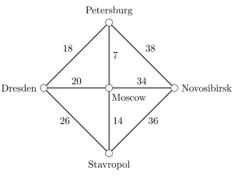
\includegraphics[scale=1.2]{images/hamiruton.JPG}
\end{figure}
使用する述語記号の表記と意味は次の通りとする。
\begin{itemize}
  \item node(X):$X$はノードである。
  \item cycle(X,Y):$XからYへ移動する。$
  \item reachable(X):ノード$X$は到達可能である。
  \item edge(X, Y):$X,Y$間に辺がある。
\end{itemize}
以下この問題における制約を示す。
\begin{enumerate}
  \item Xから移動できる場所は ちょうど 一ヶ所 (出次数=1)
  \item Xへ移動できる場所は ちょうど 一ヶ所 (入次数=1)
  \item すべてのノードは到達可能でなければいけない.
\end{enumerate}
\subsection{問題2:数独問題}
\paragraph{問題}
\begin{enumerate}
  \item 「数独」を求める問題に対する解集合プログラミング表現と、その詳細な説明
\end{enumerate}
\begin{figure}[H]
  \centering
  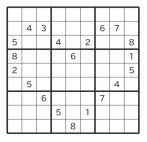
\includegraphics[scale=1.2]{images/sudoku.JPG}
\end{figure}

\section{各問の結果・考察}
\subsection{問題1:ハミルトン経路}
\paragraph{計算結果}

以下はclingoに入力するファイル「hamilton-1.lp」の内容である。
\begin{verbatim}
  node(dresden).
  node(petersburg).
  node(novosibirsk).
  node(stavropol).
  node(moscow).
  edge(stavropol, novosibirsk).
  edge(dresden, moscow).
  edge(moscow, petersburg).
  edge(dresden, petersburg).
  edge(moscow, stavropol).
  edge(dresden, stavropol).
  edge(moscow, novosibirsk).
  edge(petersburg, novosibirsk).
  edge(Y,X) :- edge(X, Y ).

  1 { cycle(X,Y) : edge(X, Y) } 1 :- node(X).
  1 { cycle(X,Y) : edge(X, Y) } 1 :- node(Y).
  reachable(Y):- cycle(s, Y).
  reachable(Y):- reachable(X), cycle(X,Y).
  :- node(X), not reachable(X).
\end{verbatim}
以下のコマンドにより、定数$s$の値を指定し、結果を得る。
\begin{itemize}
  \item ./clingo -c s=dresden hamilton-1.lp
\end{itemize}
得られた結果は下記。
\begin{verbatim}
  clingo version 5.4.0
Reading from hamilton-1.lp
Solving...
Answer: 1
edge(stavropol,novosibirsk) edge(dresden,moscow) edge(moscow,petersburg) edge(dresden,petersburg) edge(moscow,stavropol) edge(dresden,stavropol) edge(moscow,novosibirsk) edge(petersburg,novosibirsk) edge(novosibirsk,petersburg) edge(novosibirsk,moscow) edge(stavropol,dresden) edge(stavropol,moscow) edge(petersburg,dresden) edge(petersburg,moscow) edge(moscow,dresden) edge(novosibirsk,stavropol) node(dresden) node(petersburg) node(novosibirsk) node(stavropol) node(moscow) reachable(moscow) reachable(petersburg) reachable(stavropol) cycle(dresden,stavropol) reachable(novosibirsk) reachable(dresden) cycle(stavropol,moscow) cycle(petersburg,dresden) cycle(moscow,novosibirsk) cycle(novosibirsk,petersburg)
SATISFIABLE

Models       : 1+
Calls        : 1
Time         : 0.003s (Solving: 0.00s 1st Model: 0.00s Unsat: 0.00s)
CPU Time     : 0.003s

\end{verbatim}
\subsection{問題2:数独問題}

\section{まとめ}
\section{巻末資料}
本稿で使用した画像、プログラムコード等はすべて以下のリンク先に掲載している。必要に応じてご覧頂きたい。
\begin{itemize}
  \item GoogleDrive:\url{https://drive.google.com/drive/folders/1n5JPwW-wtBKLASNwndoPRlT7vyZHQvT2?usp=sharing}
  \item GitHub:\url{https://github.com/tsyu12345/logical_and_calculating_LectureCode/tree/master/No10}
\end{itemize}
\end{document}
